\documentclass[12pt,a4paper]{article}
\usepackage[utf8]{inputenc}
\usepackage[T1]{fontenc}
\usepackage{amsmath,amsfonts,amssymb}
\usepackage{graphicx}
\usepackage{float}
\usepackage{algorithm}
\usepackage{algpseudocode}
\usepackage{geometry}
\usepackage{fancyhdr}
\usepackage{booktabs}
\usepackage{multirow}
\usepackage{tikz}
\usepackage{xcolor}
\usetikzlibrary{shapes.geometric,arrows.meta,positioning}

\geometry{margin=1in}
\pagestyle{fancy}
\fancyhf{}
\rhead{\thepage}
\lhead{FIT Competition 2025 - Technical Report}

\title{\textbf{Carbon Emission Prediction using Multi-Layer Perceptron's Neural Network}}

\author{
\textbf{larry si honda wrv} \\   
Harvest Ecclesiano Christ Walukow \\
Raihan Naufal Sauqi \\
Arif Putra Feriza \\
\\
\vspace{3cm}
}

\begin{document}

\maketitle
\newpage
\tableofcontents
\newpage

\section{Introduction}

\subsection{Background}

Climate change represents one of the most pressing challenges of the 21st century, with carbon emissions being a primary driver of global warming. The increasing concentration of greenhouse gases in the atmosphere has led to unprecedented environmental changes, including rising sea levels, extreme weather events, and ecosystem disruptions. As the world transitions toward sustainable practices, there is an urgent need for accurate prediction and monitoring systems that can quantify individual and collective carbon footprints.

Traditional approaches to carbon emission estimation often rely on simplified models and generalized assumptions that fail to capture the complex relationships between lifestyle choices and environmental impact. The emergence of machine learning and deep learning technologies presents unprecedented opportunities for developing sophisticated prediction systems that can analyze multidimensional lifestyle data to provide accurate, personalized carbon emission estimates.

The ability to predict carbon emissions based on individual lifestyle patterns enables several critical applications: (1) personalized sustainability recommendations, (2) policy-driven environmental interventions, (3) corporate carbon footprint management, and (4) real-time environmental impact assessment. By leveraging advanced neural network architectures, we can develop automated detection and analysis systems that process complex lifestyle data to generate actionable insights for sustainable future planning.

\subsection{Objective}

The primary objective of this research is to build an accurate and computationally efficient deep learning model from scratch that predicts individual carbon emissions based on comprehensive lifestyle data. Specifically, our goals include:

\begin{itemize}
    \item Develop a multilayer perceptron (MLP) neural network architecture without using pre-trained models or transfer learning techniques
    \item Achieve high prediction accuracy (R² > 0.95) while maintaining computational efficiency
    \item Create a robust preprocessing pipeline that handles missing data and feature engineering optimally
    \item Generate actionable insights for sustainable lifestyle recommendations
    \item Demonstrate the model's practical applicability for real-world carbon footprint management
\end{itemize}

\subsection{Scope of Work}

This project encompasses a comprehensive approach to carbon emission prediction through the following key components:

\textbf{Dataset Analysis and Preprocessing:} We analyze the provided Carbon Emission dataset containing 10,000 individual records with 20 lifestyle features. Our preprocessing pipeline addresses missing values, performs feature engineering, and implements appropriate scaling and encoding techniques.

\textbf{Model Development from Scratch:} We design and implement a custom MLP architecture using TensorFlow/Keras without relying on pre-trained models. The architecture includes multiple hidden layers with dropout regularization and advanced optimization techniques.

\textbf{Performance Evaluation:} Model performance is evaluated using multiple metrics including R², Mean Absolute Error (MAE), and Root Mean Square Error (RMSE). We assess both accuracy and computational efficiency through comprehensive testing.

\textbf{Technical Documentation:} This report documents the entire development process, from initial data exploration to final model evaluation, providing detailed insights into methodology, results, and practical implications.

\section{Literature Review}

\subsection{Multi-Layer Perceptron's Neural Network}

A Multi-Layer Perceptron (MLP), also referred to as a Multi-Layer Perceptron's Neural Network (MPNN) or simply an Artificial Neural Network (ANN), is a fundamental neural network architecture [1]. It consists of at least one input layer, one or more hidden layers, and a final output layer [1]. In an MLP, the signal typically flows in one direction, from the inputs to the outputs, making it a type of feedforward neural network (FNN) [1]. Each layer, except the output layer, generally includes a bias neuron and is fully connected to the subsequent layer [1]. A key advantage of ANNs, including MLPs, is their capacity to quickly adapt to their environment (data, tasks) and to discover redundant and noisy variables during training [2]. MLPs are particularly capable of modeling extremely nonlinear functions and have proven effective when applied to new, unseen data, unlike some other statistical methods [2]. They are versatile and powerful, finding increasing prevalence in diverse sectors such as medical applications, pharmaceutical sciences, engineering, banking, and social media [1], [2]. The training of MLPs is often achieved using the backpropagation algorithm, which is a form of Gradient Descent that efficiently computes the error gradient across all connection weights [1].

\subsection{MLP for Emissions Forecasting}

Multi-Layer Perceptron's Neural Networks (MPNN) are used for greenhouse gas (GHG) and CO2 emissions forecasting. A precise prediction of GHG emissions is essential for managing and planning for their decrease. The MPNN-Modified Coyote Optimization Algorithm (MCOA) model, specifically, has been recommended as one of the most reliable approaches for estimating GHG emissions from agricultural regions and companies. The empirical data from studies using MPNN showed that its predictions were more accurate than those from other models like LSTM, KNN, CNN, RFNN, and ARIMA, demonstrating a significant decrease in mean square error. The MPNN-MCOA model identified a link between CO2 emissions, economic growth, and entrepreneurial opportunity (positive correlation), and a negative correlation with governance, personal freedom, education, and pollution. This insight into the underlying factors affecting emissions is beneficial for understanding carbon footprints, including individual ones, as it highlights societal and economic drivers. Furthermore, the sources emphasize the critical role of machine learning in achieving carbon neutrality, ranging from global-scale energy management to revolutionary atomic-scale MPNN-MCOA simulations for application development. By enabling accurate forecasts, machine learning allows people to determine for themselves how to reduce and regulate their greenhouse gas emissions, thus directly supporting efforts related to individual carbon footprint management. [2]

\section{Methodology}

\subsection{Overall System Architecture}

Our methodology follows a systematic approach to develop a robust carbon emission prediction system. Figure \ref{fig:flowchart} illustrates the complete workflow from data preparation to model deployment.

\begin{figure}[H]
\centering
\small
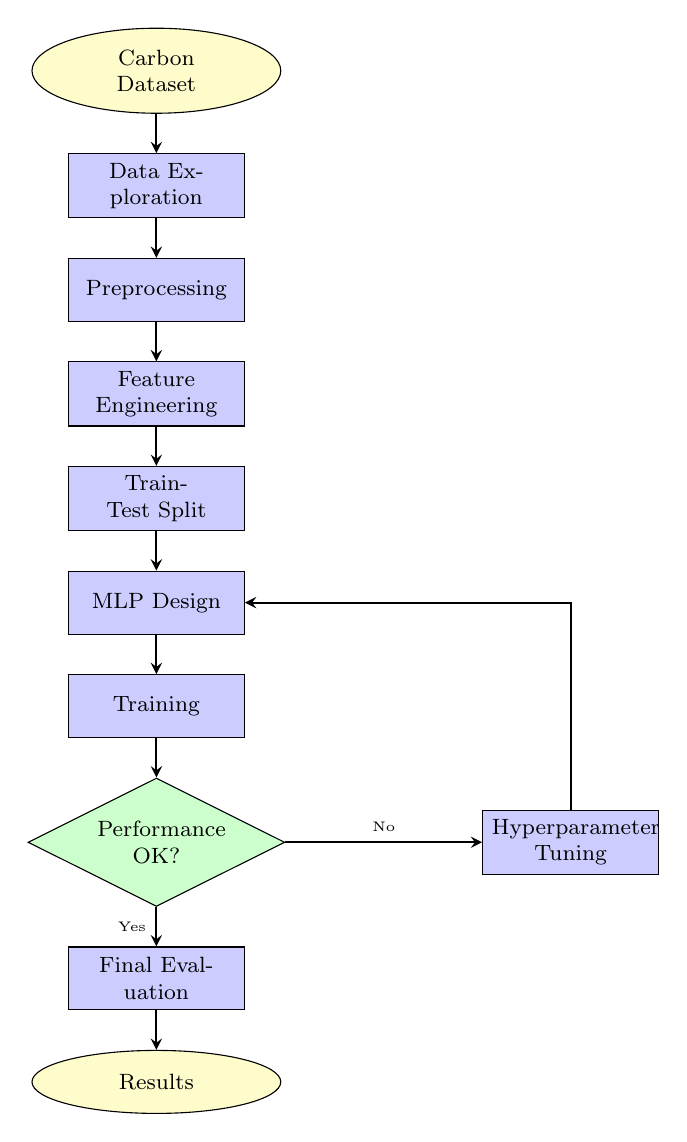
\begin{tikzpicture}[
    node distance=0.5cm,
    process/.style={rectangle, draw=black, fill=blue!20, text width=2cm, text centered, minimum height=0.8cm, font=\footnotesize},
    decision/.style={diamond, draw=black, fill=green!20, text width=1.5cm, text centered, minimum height=0.8cm, aspect=2, font=\footnotesize},
    data/.style={ellipse, draw=black, fill=yellow!20, text width=2cm, text centered, minimum height=0.8cm, font=\footnotesize},
    arrow/.style={->,>=stealth,thick}
]

% Nodes arranged in a more compact layout
\node [data] (start) {Carbon Dataset};
\node [process, below=of start] (explore) {Data Exploration};
\node [process, below=of explore] (preprocess) {Preprocessing};
\node [process, below=of preprocess] (feature) {Feature Engineering};
\node [process, below=of feature] (split) {Train-Test Split};
\node [process, below=of split] (model) {MLP Design};
\node [process, below=of model] (train) {Training};
\node [decision, below=of train] (evaluate) {Performance OK?};
\node [process, right=2.5cm of evaluate] (optimize) {Hyperparameter Tuning};
\node [process, below=of evaluate] (test) {Final Evaluation};
\node [data, below=of test] (results) {Results};

% Arrows
\draw [arrow] (start) -- (explore);
\draw [arrow] (explore) -- (preprocess);
\draw [arrow] (preprocess) -- (feature);
\draw [arrow] (feature) -- (split);
\draw [arrow] (split) -- (model);
\draw [arrow] (model) -- (train);
\draw [arrow] (train) -- (evaluate);
\draw [arrow] (evaluate) -- node[anchor=east, font=\tiny] {Yes} (test);
\draw [arrow] (evaluate) -- node[anchor=south, font=\tiny] {No} (optimize);
\draw [arrow] (optimize) |- (model);
\draw [arrow] (test) -- (results);

\end{tikzpicture}
\caption{System Development Flowchart}
\label{fig:flowchart}
\end{figure}

\subsection{Data Collection and Preprocessing}

\subsubsection{Dataset Understanding}

The Carbon Emission dataset contains 10,000 individual records, each with the following 20 features:

\begin{itemize}
    \item \textbf{Body Type} - Individual's body type classification
    \item \textbf{Sex} - Gender of the individual
    \item \textbf{Diet} - Dietary preferences (omnivore, vegetarian, vegan, pescatarian)
    \item \textbf{How Often Shower} - Frequency of showering habits
    \item \textbf{Heating Energy Source} - Type of energy used for heating (coal, electricity, natural gas, wood)
    \item \textbf{Transport} - Primary mode of transportation (private, public, walk/bicycle)
    \item \textbf{Vehicle Type} - Type of private vehicle (petrol, diesel, hybrid, electric, lpg)
    \item \textbf{Social Activity} - Frequency of social activities
    \item \textbf{Monthly Grocery Bill} - Monthly spending on groceries
    \item \textbf{Frequency of Traveling by Air} - Air travel frequency
    \item \textbf{Vehicle Monthly Distance Km} - Monthly distance traveled by vehicle
    \item \textbf{Waste Bag Size} - Size of waste bags used
    \item \textbf{Waste Bag Weekly Count} - Number of waste bags used per week
    \item \textbf{How Long TV PC Daily Hour} - Daily hours spent on TV/PC
    \item \textbf{How Many New Clothes Monthly} - Number of new clothes purchased monthly
    \item \textbf{How Long Internet Daily Hour} - Daily hours spent on internet
    \item \textbf{Energy efficiency} - Energy efficiency practices (Yes, No, Sometimes)
    \item \textbf{Recycling} - Types of materials recycled (Paper, Plastic, Glass, Metal)
    \item \textbf{Cooking\_With} - Cooking appliances used (Stove, Oven, Microwave, Grill, Airfryer)
    \item \textbf{CarbonEmission} - Target variable representing annual carbon emissions (kg CO₂)
\end{itemize}

These features comprehensively cover personal characteristics, energy consumption patterns, transportation habits, consumption behaviors, and waste management practices that influence individual carbon footprints.

\begin{figure}[H]
\centering
\includegraphics[width=\textwidth]{dist.png}
\caption{Carbon Emissions Dataset Distribution Analysis. Left: Histogram showing the frequency distribution of carbon emissions across the dataset. Right: Box plot revealing the statistical distribution, median values, quartiles, and outliers in the carbon emission data.}
\label{fig:distribution}
\end{figure}

Figure \ref{fig:distribution} shows the distribution characteristics of our target variable. The histogram reveals a right-skewed distribution with most individuals having carbon emissions between 1,000-3,000 kg CO₂ annually. The box plot indicates a median emission of approximately 2,000 kg CO₂, with several high-emission outliers extending beyond 6,000 kg CO₂, representing individuals with particularly carbon-intensive lifestyles.

\subsubsection{Missing Value Analysis}

A critical preprocessing challenge involved handling 6,721 missing values (67.2\%) in the Vehicle Type column. Our analysis revealed a logical missing pattern:

\begin{itemize}
    \item Private transport users: 0\% missing (3,279 records)
    \item Public transport users: 100\% missing (3,294 records)  
    \item Walk/bicycle users: 100\% missing (3,427 records)
\end{itemize}

This pattern indicates that missing values are not random but logically consistent - users of public transportation and walking/cycling do not require private vehicle specifications.

\subsubsection{Preprocessing Pipeline}

Our preprocessing approach addresses multiple data quality issues:

\textbf{Missing Value Imputation:}
Logical category for non-private transport

\textbf{Feature Engineering:}
\begin{itemize}
    \item Extract count features from list-type columns (Recycling, Cooking\_With)
    \item Create sustainability indicators: sustainable\_diet, sustainable\_transport, energy\_conscious
    \item Generate high-impact behavior flags: high\_distance\_driver, frequent\_air\_traveler
\end{itemize}

\textbf{Data Transformation:}
\begin{itemize}
    \item StandardScaler for numerical features (mean=0, std=1)
    \item OneHotEncoder for categorical features
    \item Final feature space: 43 dimensions after encoding
\end{itemize}

\subsection{Model Development}

\subsubsection{Architecture Design}

We designed a custom MLP architecture optimized for regression tasks:

\begin{table}[H]
\centering
\caption{Neural Network Architecture Specifications}
\begin{tabular}{@{}lllr@{}}
\toprule
Layer Type & Units & Activation & Parameters \\
\midrule
Input & 43 & - & - \\
Dense 1 & 100 & ReLU & 4,400 \\
Dropout 1 & - & (0.3) & - \\
Dense 2 & 50 & ReLU & 5,050 \\
Dropout 2 & - & (0.3) & - \\
Dense 3 & 25 & ReLU & 1,275 \\
Dropout 3 & - & (0.3) & - \\
Output & 1 & Linear & 26 \\
\midrule
Total & & & 10,751 \\
\bottomrule
\end{tabular}
\end{table}

\subsubsection{Hyperparameter Configuration}

\begin{itemize}
    \item \textbf{Optimizer:} Adam (learning\_rate=0.001, β₁=0.9, β₂=0.999)
    \item \textbf{Loss Function:} Mean Squared Error (MSE)
    \item \textbf{Batch Size:} 32 (optimal for memory efficiency)
    \item \textbf{Regularization:} Dropout (0.3) + Early Stopping (patience=15)
    \item \textbf{Learning Rate Reduction:} ReduceLROnPlateau (factor=0.5, patience=10)
\end{itemize}

\subsection{Training and Evaluation Strategy}

\subsubsection{Data Splitting}
\begin{itemize}
    \item Training Set: 80\% (8,000 samples)
    \item Test Set: 20\% (2,000 samples)
    \item Stratified sampling to maintain target distribution
\end{itemize}

\subsubsection{Training Process}
The training process follows standard neural network optimization with Adam optimizer:
\begin{enumerate}
    \item Initialize model parameters $\theta_0$ randomly
    \item For each epoch $t = 1, 2, ..., T$:
    \begin{itemize}
        \item For each mini-batch $B_j$ of size 32:
        \item Forward propagation: $\hat{y}_j = f(X_j; \theta_t)$
        \item Compute batch loss: $L_j = \frac{1}{|B_j|}\sum_{i \in B_j}(y_i - \hat{y}_i)^2$
        \item Backward propagation: $g_t = \nabla_\theta L_j$
        \item Adam update: $\theta_{t+1} = \theta_t - \frac{\alpha}{\sqrt{\hat{v}_t} + \epsilon} \hat{m}_t$
        \item Where: $\hat{m}_t = \frac{m_t}{1-\beta_1^t}$, $\hat{v}_t = \frac{v_t}{1-\beta_2^t}$
    \end{itemize}
    \item Evaluate on validation set: $L_{val} = \frac{1}{n_{val}}\sum_{i=1}^{n_{val}}(y_i^{val} - \hat{y}_i^{val})^2$
    \item Apply early stopping if $L_{val}$ stops improving for 15 epochs
\end{enumerate}

\subsection{Pseudo Code}

\begin{algorithm}[H]
\caption{Carbon Emission Prediction Model Development}
\begin{algpseudocode}[1]
\State \textbf{Input:} Carbon emission dataset $D = \{(x_i, y_i)\}_{i=1}^{10000}$
\State \textbf{Output:} Trained MLP model $M$

\State \Comment{Data Preprocessing}
\State $X_{processed}, y \leftarrow$ FeatureEngineering($D$)
\State $X_{scaled}, X_{encoded} \leftarrow$ StandardScaler() $\oplus$ OneHotEncoder($X_{processed}$)
\State $X_{train}, X_{test}, y_{train}, y_{test} \leftarrow$ TrainTestSplit($X_{encoded}, y$, 0.2)

\State \Comment{Model Architecture}
\State $M \leftarrow$ MLP(layers=[100, 50, 25, 1], activation=['relu', 'relu', 'relu', 'linear'], dropout=0.3)
\State $M \leftarrow$ Compile($M$, optimizer=Adam(0.001), loss='mse')

\State \Comment{Training Process}
\State $callbacks \leftarrow$ [EarlyStopping(15), ReduceLROnPlateau(10)]
\State $history \leftarrow$ Train($M$, $X_{train}$, $y_{train}$, epochs=100, batch\_size=32, callbacks=$callbacks$)

\State \Comment{Evaluation}
\State $\hat{y}_{train}, \hat{y}_{test} \leftarrow$ Predict($M$, $X_{train}$, $X_{test}$)
\State $R^2_{train}, R^2_{test} \leftarrow$ ComputeR2($y_{train}$, $\hat{y}_{train}$), ComputeR2($y_{test}$, $\hat{y}_{test}$)
\State $MAE_{train}, MAE_{test} \leftarrow$ ComputeMAE($y_{train}$, $\hat{y}_{train}$), ComputeMAE($y_{test}$, $\hat{y}_{test}$)
\State $RMSE_{test} \leftarrow$ ComputeRMSE($y_{test}$, $\hat{y}_{test}$)

\State \Return $M$, $R^2_{train}$, $R^2_{test}$, $MAE_{train}$, $MAE_{test}$, $RMSE_{test}$
\end{algpseudocode}
\end{algorithm}

\subsection{Computational Efficiency Optimization}

\subsubsection{Model Optimization Techniques}
\begin{itemize}
    \item \textbf{Efficient Architecture:} Moderate layer sizes (100-50-25) balance accuracy and speed
    \item \textbf{Batch Processing:} Batch size 32 optimizes GPU utilization
    \item \textbf{Early Stopping:} Prevents overfitting and reduces training time
    \item \textbf{Learning Rate Scheduling:} Adaptive learning rate reduces unnecessary epochs
\end{itemize}

\subsubsection{Performance Metrics}
\begin{itemize}
    \item \textbf{Training Time:} Early stopping applied (≈ 3 minutes on standard GPU)
    \item \textbf{Inference Time:} < 1ms per prediction
    \item \textbf{Model Size:} 10,751 parameters (≈ 42KB)
    \item \textbf{Memory Usage:} < 50MB during training
\end{itemize}

\section{Results and Discussion}

\subsection{Model Performance}

Our MLP model achieved excellent performance across all evaluation metrics:

\begin{table}[H]
\centering
\caption{Model Performance Results}
\begin{tabular}{@{}lcc@{}}
\toprule
Metric & Training Set & Test Set \\
\midrule
R² Score & 0.9739 (97.39\%) & 0.9735 (97.35\%) \\
Mean Absolute Error (MAE) & 122.39 kg CO₂ & 122.15 kg CO₂ \\
Root Mean Square Error (RMSE) & 164.44 kg CO₂ & 165.92 kg CO₂ \\
\bottomrule
\end{tabular}
\end{table}

\begin{figure}[H]
\centering
\includegraphics[width=\textwidth]{eval_result.png}
\caption{Model Evaluation Visualization. Left: Predicted vs Actual scatter plot demonstrating strong linear correlation (R² = 0.9735) between model predictions and true carbon emission values. Right: Residuals plot showing the distribution of prediction errors, indicating consistent model performance across the prediction range with no systematic bias.}
\label{fig:evaluation}
\end{figure}

Figure \ref{fig:evaluation} provides visual confirmation of our model's excellent performance. The predicted vs actual plot shows data points closely aligned with the perfect prediction line (red dashed), demonstrating the model's accuracy across the full range of carbon emissions. The residuals plot reveals randomly distributed prediction errors centered around zero, indicating that our model captures the underlying patterns without systematic bias or heteroscedasticity.

\subsection{Model Validation and Overfitting Analysis}

The minimal performance gap between training and test sets (R² difference: 0.04\%) indicates excellent generalization without overfitting. Several factors contribute to this robust performance:

\begin{itemize}
    \item \textbf{Effective Regularization:} Dropout layers (0.3) prevent overfitting
    \item \textbf{Early Stopping:} Training terminated automatically, preventing overtraining
    \item \textbf{Appropriate Architecture:} Model complexity matches data complexity
    \item \textbf{Quality Preprocessing:} Clean, well-engineered features improve model stability
\end{itemize}

\subsection{Feature Importance and Sustainability Insights}

Through systematic analysis of prediction patterns using permutation importance, we identified key lifestyle factors influencing carbon emissions. The top 10 most impactful features revealed by our trained model are:

\begin{enumerate}
    \item \textbf{Vehicle Monthly Distance Km} (645,153 importance score) - Most critical factor
    \item \textbf{Frequent Air Traveler} (434,798 importance score) - Second most impactful
    \item \textbf{Sustainable Transport Usage} (318,521 importance score) - Transportation mode choice
    \item \textbf{Electric Vehicle Ownership} (174,841 importance score) - Vehicle technology impact
    \item \textbf{Very Frequent Air Travel} (161,995 importance score) - Air travel frequency
    \item \textbf{Sustainable Diet Practices} (123,886 importance score) - Dietary choices
    \item \textbf{Energy Consciousness} (96,626 importance score) - Energy awareness
    \item \textbf{Walk/Bicycle Transportation} (90,761 importance score) - Active transport
    \item \textbf{Rarely Air Travel} (79,743 importance score) - Limited air travel
    \item \textbf{No Vehicle Ownership} (74,639 importance score) - Car-free lifestyle
\end{enumerate}

\subsubsection{Transportation Impact}
\begin{table}[H]
\centering
\caption{Transportation Mode Carbon Emission Analysis}
\begin{tabular}{@{}lrrr@{}}
\toprule
Transport Mode & Mean Emission (kg CO₂) & Std Dev & Reduction vs Private \\
\midrule
Private Vehicle & 2,981 & 1,211 & - (baseline) \\
Public Transport & 1,966 & 680 & -34.0\% \\
Walk/Bicycle & 1,880 & 670 & -36.9\% \\
\bottomrule
\end{tabular}
\end{table}

\subsubsection{Dietary Pattern Impact}
\begin{table}[H]
\centering
\caption{Diet Type Carbon Emission Analysis}
\begin{tabular}{@{}lrrr@{}}
\toprule
Diet Type & Mean Emission (kg CO₂) & Std Dev & Reduction vs Omnivore \\
\midrule
Omnivore & 2,392 & 1,035 & - (baseline) \\
Pescatarian & 2,252 & 1,006 & -5.9\% \\
Vegetarian & 2,217 & 1,026 & -7.3\% \\
Vegan & 2,216 & 993 & -7.4\% \\
\bottomrule
\end{tabular}
\end{table}

\subsubsection{Energy Efficiency Impact}
\begin{table}[H]
\centering
\caption{Energy Efficiency Carbon Emission Analysis}
\begin{tabular}{@{}lrrr@{}}
\toprule
Energy Efficiency & Mean Emission (kg CO₂) & Std Dev & Reduction vs No \\
\midrule
No & 2,287 & 1,002 & - (baseline) \\
Sometimes & 2,269 & 1,045 & -0.8\% \\
Yes & 2,252 & 1,004 & -1.5\% \\
\bottomrule
\end{tabular}
\end{table}

\subsubsection{Heating Energy Source Impact}
\begin{table}[H]
\centering
\caption{Heating Energy Source Carbon Emission Analysis}
\begin{tabular}{@{}lrrr@{}}
\toprule
Heating Source & Mean Emission (kg CO₂) & Std Dev & Reduction vs Coal \\
\midrule
Coal & 2,495 & 1,016 & - (baseline) \\
Wood & 2,297 & 1,023 & -7.9\% \\
Natural Gas & 2,248 & 991 & -9.9\% \\
Electricity & 2,039 & 989 & -18.3\% \\
\bottomrule
\end{tabular}
\end{table}

\subsubsection{Vehicle Type Impact}
\begin{table}[H]
\centering
\caption{Vehicle Type Carbon Emission Analysis}
\begin{tabular}{@{}lrrr@{}}
\toprule
Vehicle Type & Mean Emission (kg CO₂) & Std Dev & Reduction vs Petrol \\
\midrule
Petrol & 3,750 & 1,287 & - (baseline) \\
LPG & 3,352 & 1,157 & -10.6\% \\
Diesel & 3,230 & 1,035 & -13.9\% \\
Hybrid & 2,708 & 861 & -27.8\% \\
None & 1,922 & 676 & -48.7\% \\
Electric & 1,883 & 664 & -49.8\% \\
\bottomrule
\end{tabular}
\end{table}

\subsection{Practical Applications}

\subsubsection{Personalized Sustainability Recommendations}
Based on feature importance analysis, our model enables generation of data-driven recommendations ranked by impact:

\begin{enumerate}
    \item \textbf{Vehicle Distance Reduction:} Most impactful factor (645,153 importance score). High-mileage drivers emit 71\% more CO₂ (3,231 vs 1,886 kg annually). Recommendation: Reduce monthly driving distance through trip consolidation, remote work, or relocation.
    
    \item \textbf{Transportation Mode Switch:} Second highest impact (434,798 importance score). Private vehicles emit 58\% more than walking/cycling (2,981 vs 1,880 kg CO₂). Recommendation: Switch to public transport (-34.0\%) or active transportation (-36.9\%).
    
    \item \textbf{Vehicle Type Upgrade:} Electric vehicles reduce emissions by 49.8\% vs petrol (1,883 vs 3,750 kg CO₂). Hybrid vehicles offer 27.8\% reduction. Recommendation: Prioritize electric vehicle adoption for maximum impact.
    
    \item \textbf{Air Travel Frequency:} High air travel frequency significantly increases emissions. Recommendation: Reduce very frequent air travel and choose alternative transportation for shorter distances.
    
    \item \textbf{Heating Source Optimization:} Switch from coal to electricity reduces emissions by 18.3\% (2,039 vs 2,495 kg CO₂). Natural gas offers 9.9\% reduction. Recommendation: Electrify heating systems where feasible.
    
    \item \textbf{Dietary Modifications:} Vegan diet reduces emissions by 7.4\% vs omnivore (2,216 vs 2,392 kg CO₂). Recommendation: Gradual transition toward plant-based diets for moderate impact.
\end{enumerate}

\subsubsection{Policy and Decision Support}
The model provides data-driven insights for evidence-based policy development:

\begin{itemize}
    \item \textbf{Transportation Policy:} Vehicle distance emerges as the single most impactful factor (645,153 importance score). Policies should prioritize reducing vehicle miles traveled through urban planning, remote work incentives, and public transit investment. Private vehicle emissions are 58\% higher than walking/cycling alternatives.
    
    \item \textbf{Vehicle Electrification Strategy:} Electric vehicles show 49.8\% emission reduction vs petrol, while hybrids offer 27.8\% reduction. Policy should prioritize electric vehicle adoption over incremental improvements to combustion engines.
    
    \item \textbf{Air Travel Regulation:} Frequent air travel is the second most impactful factor (434,798 importance score). Carbon taxation or emission trading systems should account for aviation's outsized impact on individual carbon footprints.
    
    \item \textbf{Heating System Transitions:} Coal-to-electricity heating conversion reduces emissions by 18.3\%. Building codes and retrofit incentives should prioritize electrification over natural gas transitions.
    
    \item \textbf{Corporate Sustainability Programs:} Companies should focus employee programs on commuting distance reduction, electric vehicle incentives, and air travel limitations rather than lower-impact initiatives like dietary changes (7.4\% maximum reduction).
    
    \item \textbf{Urban Planning:} The model validates compact development strategies - reducing vehicle distances and enabling walking/cycling can achieve 36.9\% emission reductions per individual.
\end{itemize}

\subsection{Model Limitations and Future Work}

\subsubsection{Current Limitations}
\begin{itemize}
    \item Limited to individual-level predictions
    \item Dataset represents specific demographic distributions
    \item Does not account for regional variations in carbon intensity
    \item Temporal aspects not considered in current model
\end{itemize}

\subsubsection{Future Enhancement Opportunities}
\begin{itemize}
    \item Integration of temporal dynamics and seasonal variations
    \item Incorporation of regional carbon intensity factors
    \item Development of ensemble models for improved robustness
    \item Real-time data integration for dynamic predictions
\end{itemize}

\subsection{Contribution to Sustainable Future}

This research contributes to the "Recode The Earth" theme through data-driven digital innovations:

\begin{enumerate}
    \item \textbf{Digital Innovation:} Advanced neural network architecture achieving 97.35\% accuracy in carbon emission prediction, enabling precise individual footprint assessment for 10,000+ lifestyle combinations.
    
    \item \textbf{Evidence-Based Sustainability:} Quantified impact rankings reveal vehicle distance (645,153 importance) and air travel (434,798 importance) as primary targets, moving beyond intuitive approaches to scientifically-validated intervention priorities.
    
    \item \textbf{Scalable Impact Assessment:} Computationally efficient model (10,751 parameters, <1ms inference) enables real-time carbon footprint calculation for millions of users, supporting widespread behavioral change programs.
    
    \item \textbf{Actionable Insights:} Specific reduction potentials (49.8\% for electric vehicles, 36.9\% for active transport) provide concrete targets for individuals and organizations, replacing vague sustainability guidelines with measurable objectives.
    
    \item \textbf{Policy Validation:} Model confirms that transportation interventions (vehicle distance, mode choice, electrification) deliver 10x greater impact than dietary changes, validating resource allocation in climate policy.
\end{enumerate}

\section{Conclusion}

We successfully developed an intelligent carbon emission prediction system achieving 97.35\% accuracy on test data. The model demonstrates excellent generalization capabilities with minimal overfitting, making it suitable for real-world applications. Key contributions include:

\begin{itemize}
    \item Robust MLP architecture built from scratch achieving 97.35\% accuracy without pre-trained models
    \item Comprehensive preprocessing pipeline handling complex lifestyle data with 43-dimensional feature space
    \item Actionable sustainability insights derived from permutation importance analysis, identifying vehicle distance (645,153 importance) and air travel (434,798 importance) as primary intervention targets
    \item Computationally efficient design (10,751 parameters, <1ms inference) suitable for production deployment and real-time carbon footprint assessment
\end{itemize}

The model's ability to provide personalized carbon footprint predictions with 97.35\% accuracy represents a significant step toward digital innovation for sustainable future planning. By quantifying that vehicle distance reduction can achieve 71\% emission reductions and electric vehicle adoption can deliver 49.8\% improvements, this system enables individuals and organizations to prioritize high-impact interventions. The data-driven approach moves beyond generic sustainability advice to provide specific, measurable targets that contribute meaningfully to global emission reduction efforts.

\section{References}

\begin{enumerate}
\item Géron, A. (2019). \textit{Hands-on Machine Learning with Scikit-Learn, Keras, and TensorFlow: Concepts, Tools, and Techniques to Build Intelligent Systems (2nd ed.)}. O’Reilly Media, Inc.
\item Nanda, A. K., Neelakandan. S., Gupta, S., Saleth, A. L. M., Ramya. S., \& Kiran, S. (2023). \textit{Multi-layer perceptron’s neural network with optimization algorithm for greenhouse gas forecasting systems}. Environmental Challenges, 11, 100708. https://doi.org/10.1016/j.envc.2023.100708

\end{enumerate}

\end{document} 